\documentclass{article}
\usepackage{graphicx}
\usepackage{hyperref}
\usepackage[utf8]{inputenc}
\usepackage{lipsum}
\usepackage{courier} %% Sets font for listing as Courier.
\usepackage{listings, xcolor}
\usepackage{biblatex}
\usepackage{longtable}
\addbibresource{test.bib}

\lstset{
tabsize = 4, %% set tab space width
showstringspaces = false, %% prevent space marking in strings, string is defined as the text that is generally printed directly to the console
numbers = left, %% display line numbers on the left
commentstyle = \color{green}, %% set comment color
keywordstyle = \color{blue}, %% set keyword color
stringstyle = \color{red}, %% set string color
rulecolor = \color{black}, %% set frame color to avoid being affected by text color
basicstyle = \ttfamily , %% set listing font and size
breaklines = true, %% enable line breaking
numberstyle = \tiny,
}

\title{Software Testing Project}
\author{
  Mark Reilly\\
  \href{https://github.com/MarkReillyGMIT}{Github}
}
\date{\today}

\begin{document}

\begin{figure}
    \centering
    
\includegraphics[scale=0.3]{./images/gmit.jpg}
\end{figure}

\maketitle


\tableofcontents
\newpage


\section{Introduction}
\subsection{Document Purpose}
This document is a high-level overview defining our testing strategy for Game Development Ltd  new 2D side-scrolling plat-former.The 
objective of the game is for the player to navigate through progressively difficult levels.The test team will verify the quality of the product prior to release. The document also lists the different resources that are needed for a successful testing of the project.

\subsection{High Level Functions:}
\begin{enumerate}
    \item Unit Testing
    \item Integration Testing
    \item Smoke  Testing
    \item Regression  Testing
    \item Sanity  Testing
    \item User Acceptance Testing
\end{enumerate}

\subsection{Document Audience}
Business owner(s), stakeholders and project team members are the intended audience for this document. Stakeholders will be requested to provide feedback on the overall scope of the test effort and any omissions.


\newpage

\section{OBJECTIVES AND TASKS}

\subsection{Objectives}
The objective of our test plan is to find and report as many bugs as possible to improve the integrity of our product. We will use a broad range of tests to achieve our goals. The test plan document supports the following objectives:
\begin{enumerate}
    \item Identify existing project information and the software that            should be tested.
    \item List the recommended test requirements (high level).
    \item Recommend and describe the testing strategies to be employed.
    \item Identify the required resources and provide an estimate of the         test efforts.
    \item List the deliverable elements of the test activities.
\end{enumerate}
\subsection{Tasks}
\begin{enumerate}
    \item Identify what particular tests will be used to test each module.
    \item Identify the expected results for each test.
    \item Perform the tests.    
    \item Document the test data, test cases and test configuration used during the testing process.
    \item Successful unit testing is required before it is eligible for system and integration testing.
    \item Unsuccessful testing will require a Bug Report to be generated.
    \item Test documents and reports should be submitted when all is complete.
\end{enumerate}

\newpage

\section{Scope}
\subsubsection{General}
The main components of the game that need to be tested are as follows:
\begin{enumerate}
    \item Main Menu:
    
    The Main Menu will have three options on start-up: ‘Play’, ‘Settings’, and ‘Exit Game’.
    Selecting ‘Play’ will take the player into the game and the player will begin at Level 1.
    If a save system is able to be implemented, the player will begin at their last saved
    point. ‘Settings’ will allow the player to edit game settings, such as sound level and
    music level. ‘Exit Game’ will quit the application’.
    \item Player Movement:
    
    Player Movement will be tested to see if the player is able to move the character, also to see if the player is confined to the screen and not able to go out of view and disappear.The players jump, crouch and attack abilities will be tested under this section.
    \item Player Health Counter:
    
    The players health counter will be tested to see if the player loses a life after being hit by an enemy. When the player collects an extra health, the health counter should go up by one.If the player loses all of its lives, it should be destroyed.
    \item Enemy Health Counter:
    
    The enemies health counter will be tested to see if the enemy loses a life after being hit by the players bullet.When the enemy loses all its lives, the enemy should be destroyed. If the enemy is the boss enemy at the end of each level and it is destroyed , the player should be brought to the next level.
    \item In-Game Menu:
    
    The game will include a number of options when the game is paused, similar to those
    available on start up. The player will be able to resume the game, access settings,
    restart the level, and exit the game. All the in-game menu options will be tested to see if the selected options does its intended function.
    
\end{enumerate}
\subsubsection{Tactics:}
\begin{figure}
    \centering
    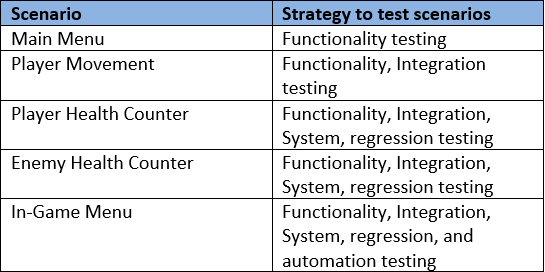
\includegraphics[scale=0.9]{./images/tactics.PNG}
\end{figure}

\newpage

\section{Testing Strategy}

\subsection{Unit Testing}
\subsubsection{Definition}
UNIT TESTING is a level of software testing where individual units/ components of a software are tested. The purpose is to validate that each unit of the software performs as designed.
\subsubsection{Participants}
Developers
\subsubsection{Methodology}
Unit test case has been processed by Developers and they will write the test scripts for the unit testing if game.
\centering
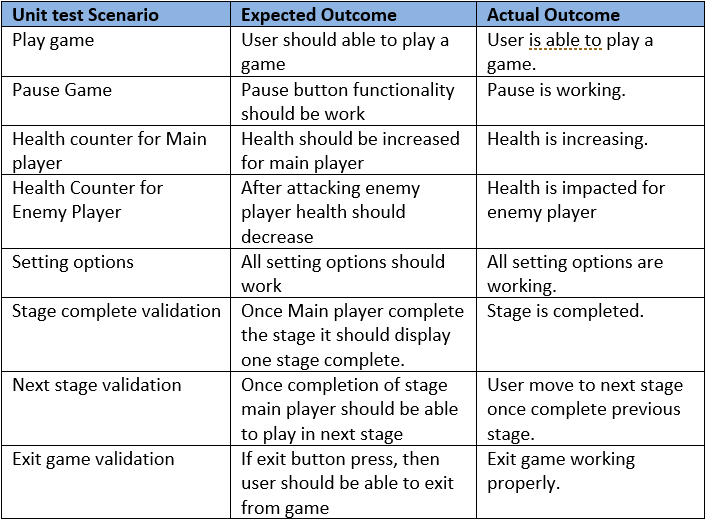
\includegraphics[scale=0.9]{./images/unittesting.PNG}


\subsection{System and Integration Testing}
\subsection{Performance and Stress Testing}
\subsection{User Acceptance Testing }
\subsection{Batch Testing}
\subsection{Automated Regression Testing }
\subsection{Beta Testing Participants}

\newpage

\section{Testing Schedule}

\newpage

\section{Control Procedures}

\newpage

\section{Features to be Tested}

\newpage

\section{Features not to be Tested}

\newpage

\section{Roles & Responsibilities}
\begin{itemize}
    \item Game producers are responsible for setting testing deadlines in coordination with marketing and quality assurance.They also manage many items outside of game testing, relating to the overall production of a title. Their approval is typically required for final submission.
    \item Lead tester, test lead or QA lead is the person responsible for the game working correctly and managing bug lists. A lead tester manages the QA staff. Lead tester works closely with designers and programmers, especially towards the end of the project. The lead tester is responsible for tracking bug reports and managing that they are fixed. They are also responsible that QA teams produce formal and complete reports.
    \item Testers are responsible for checking that the game works, is easy to use, has actions that make sense, and contains fun game play. Testers need to write accurate and specific bug reports, and if possible providing descriptions of how the bug can be reproduced. Testers may be assigned to a single game during its entire production, or brought onto other projects as demanded by the department's schedule and specific needs.
\end{itemize}
\newpage

\section{Schedules}

\newpage

\section{Risks/Assumptions}
\begin{table}[h!]
\centering
 \begin{tabular}{||c{1cm} c||} 
 \hline
 Risk & Mitigation Strategy \\ [0.5ex] 
 \hline
 \hline
 Late submission of information,\\ delays in document approval by the Customer & Scheduling of meetings and the provision of \\ & necessary information for deadlines\\ [1ex] 
 \hline
 \end{tabular}
\end{table}
\newpage

\section{Tools}

\newpage

\end{document}
